\section{Umsetzungsplanung - CH}
\todo[inline]{Ich bin ein einleitender Text, der noch geschrieben werden muss.}

\subsection{Positionsbestimmung}
Für einen erfolgreichen Umsetzungsplan mit der Zielsetzung einer Neuordnung des Informationsmanagements an einer Hochschule ist eine Positionsbestimmung der aktuellen Situation von elementarer Bedeutung. Hierzu muss der Ist-Zustand des aktuellen Informationsmanagements mit der Zielformulierung des avisierten Informationsmanagements an der Hochschule erfasst und abgeglichen werden. 

Da solche Veränderungen in der Regel einen langwierigen Prozess darstellen, ist es ratsam, Prioritäten zu definieren und die einzelnen Teilbereiche anhand der Dringlichkeit umzusetzen.

Ist die Position bestimmt, kann davon ausgehend ein entsprechender Migrationsplan (vgl. Kapitel \ref{section_migrationskonzepte}) und, wenn noch nicht geschehen, ein Changeplan (vgl. Kapitel \ref{subsection_change_management}) erstellt werden. Je nach Art und Umfang der Veränderungen sollte allerdings das Change Management nicht erst nach der Positionsbestimmung angewandt werden, sondern schon bei der Zielbestimmung – also mit in die Erarbeitung des möglichen Soll-Zustands einfliessen.

Diese Ausarbeitung wird sich aus Gründen der Komplexität im praxisbezogenen Teil nicht auf das gesamte Informationsmanagement der Hochschule Emden/Leer beziehen können. Exemplarisch wird daher eine Umsetzungsplanung an den Beispielen des Dokumentenmanagements Alfresco und der Erstellung eines responsive Designs der Webpräsenz der Hochschule erarbeitet.

Alfresco wird derzeit noch nicht an der Hochschule eingesetzt. Zur Zeit werden Dokumente in verschieden Systemen verwaltet und zugäglich gemacht. Für die Webpräsenz wird derzeit ein TYPO3-System in der Version 4.5 LTS (Long Term Support) genutzt, welches noch nicht für mobile Endgeräte optimiert ist.

\subsection{Change Management}
\label{subsection_change_management}

\todo[inline]{Ich bin ein einleitender Text, der noch geschrieben werden muss.}

\subsubsection{Grundlagen des Change Managements}
Die Umsetzung einer Neuordnung des Informationsmanagements an einer Hochschule bedeutet auch Wandel und Veränderungen. Um das optimal zu steuern, bedarf es spezieller Managementtechniken, welche sich unter dem Begriff Change Management zusammenfassen lassen. Im Vordergrund aller Betrachtungen steht der Faktor Mensch, denn für eine erfolgreiche Umsetzung von Veränderungen ist die aktive Unterstützung der Betroffenen von erheblicher Bedeutung.\footnote{\cite{lauer_change_2014}}

\begin{figure}[h!]
	\centering
	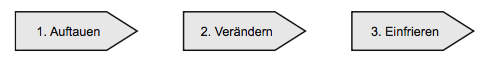
\includegraphics[width=10cm]{kapitel/gruppe4_1/bilder/drei_phasen_modell}
	\caption{3-Phasen-Modell nach Kurt Lewin}
	\label{fig_drei_phasen_modell}
\end{figure}

\begin{itemize}
	\item Die Betroffenen sollen Veränderungen motiviert werden.
	\item Die Betroffenen sollen für Veränderungen trainiert werden und der Veränderungsprozess vollzogen werden.
	\item Die die Veränderungen sollen Stabilisiert werden.
\end{itemize}


Nach Thomas Lauer sollte das Change Management grundsätzlich an drei Punkten ansetzen:
\begin{itemize}
	\item \textbf{Individuum:} Das Individuum beschreibt jeden Einzelnen. Ohne die Mitarbeit der Betroffenen ist ein Wandel unmöglich. Das Change Management soll nicht nur die Fähigkeiten des Einzelnen an neue Herausforderungen anpassen, sondern auch die positive Einstellung gegenüber der Ziele des Wandels aller Betroffenen fördern.
	\item \textbf{Unternehmensstruktur (bzw. Hochschulstruktur):} Die Unternehmensstruktur umfasst Aufbau- und Ablauforganisation sowie Strategien und Ressourcen. Veränderungen in diesen Bereichen sind auf dem Papier grundsätzlich einfach.
	\item \textbf{Unternehmenskultur (bzw. Hochschulkultur):} Die Unternehmenskultur beschreibt dauerhafte, über lange Zeit gewachsene Strukturen die für Einstellung, Werte und Regeln des Umgangs verantwortlich sind. 
\end{itemize}

In den meisten Fällen bringt ein Wandel in den oben genannten Bereichen Veränderungen in allen Dimensionen mit sich, die sich wechselseitig beeinflussen.\footnote{\cite{fisch_veraenderungen_2008}} 

So ist z. B. ein Wandel ohne die Einbeziehung der Unternehmenskultur oftmals zum scheitern verurteilt.\footnote{\cite{lauer_change_2014}} Das heißt, für ein erfolgreiches Change Management sollten grundsätzlich die Abhängigkeiten der Bereiche untereinander berücksichtigt werden.

Veränderungen bedeuten Neues und Ungewohntes für alle Betroffenen. 
Betroffene müssen veränderte Aufgaben erledigen, neue Technologien und Methoden erlernen, erneut soziale Beziehungen zu Kollegen, Vorgesetzten oder Kunden aufbauen, mit Problemen in der Implementierungsphase umgehen und ggf. ihre Werte in Einklang mit neuen Standards und Zielen der Organisation bringen.\footnote{\cite{fisch_veraenderungen_2008}}

Dies kann zu Zweifeln und Widerständen führen, was im schlimmsten Fall ein Scheitern des gesamten Vorhabens bedeuten kann. Als Ursache eines gescheiterten Wandels steht der Widerstand an oberster Stelle. Mangelhafte Prozessteuerung, zu schnelles Veränderungstempo und unklare Zielsetzungen spielen dabei ein wichtige Rolle und können Gründe für eben diesen Widerstand sein.\footnote{\cite{lauer_change_2014}}

Die Bereitschaft zum Wandel nimmt zu, wenn die Betroffenen überzeugt sind, das die Veränderungen ihnen persönlich nutzen, ihre Identität nicht bedroht ist und ihre Werte und Ziele mit dem Wandel in Einklang gebracht werden können.

Des weiteren wird die Bereitschaft zum Wandel gefördert wenn die Betroffenen über Fähigkeiten verfügen, die den veränderten Anforderungen gerecht werden. Die Aufgabe des Change Management ist es, durch Information, Partizipation, Unterstützung (z. B. Coaching) und Anreizgestaltung den Betroffenen die Zweifel und Unsicherheit zu nehmen.\footnote{\cite{fisch_veraenderungen_2008}} 

\begin{itemize}
\item \textbf{Kommunikation}
Nach Thomas Lauer ist einer der entscheidendsten Erfolgsfaktoren des Change Managements die Kommunikation. Kommunikation schafft Transparenz und damit Orientierung und dient damit auch der Beilegung von Widerständen. Damit ist aber auch ein potenzieller Misserfolg eines Change Managements auf die Kommunikation zurückzuführen. Fehlinterpretationen und Missverständnisse können schnell zu Konflikten führen.\footnote{\cite{lauer_change_2014}}

Es sollten also entsprechende Kommunikationsstrategien und Kommunikationspläne erarbeitet werden, um die Betroffenen für die Veränderungen zu gewinnen und Missverständnissen aus dem Weg zu gehen. In der Startphase sollten die Betroffenen über Gründe, Ziele, Notwendigkeit, Nutzen und den zeitlichen Ablauf informiert werden. Aber auch potentielle Risiken und Schwierigkeiten sollten von Anfang an offen kommuniziert werden.\footnote{\cite{fisch_veraenderungen_2008}}

In der Durchführungsphase ist es wichtig die Kommunikation aufrecht zu erhalten. Beispielsweise können Projektfortschritte regelmäßig an alle Betroffenen weitergegeben werden. Durch das Aufrechterhalten der Kommunikation können frühzeitig Widerstände erkannt und überwunden werden.\footnote{\cite{lauer_change_2014}} 

\item \textbf{Partizipation}
Ein weiterer wichtiger Erfolgsfaktor ist die Partizipation. Das Einbinden möglichst vieler Betroffenen in den Change Prozess erhöht die Motivation und hilft den Betroffenen sich mit den Veränderungen zu identifizieren. Haben Betroffene andere Positionen oder Sichtweisen gegenüber des Wandels als die Organisation müssen diese Widerstände nicht gleich negativ ausgelegt werden. Die Ideen und Vorschläge der Betroffenen können in den Change Prozess einfliessen und weiterhin Veränderungen optimieren.

\item \textbf{Unterstützung}:
Besonders wenn es um neue Technologien, Werkzeuge oder Verfahren geht, ist Unterstützung für die Betroffenen gefordert. Die Unterstützung hat zum Ziel, die Betroffenen des Wandels auf die zusätzlichen oder neuen Anforderungen vorzubereiten. In den Meisten Fällen geschieht das in Form von Weiterbildung oder Coaching.

Des weiteren fördert eine vom Unternehmen ausgehende Weiterbildung nicht nur den Aufbau von Qualifikationen und die Erweiterung des Wissens der Betroffenen, sondern auch die Motivation. Den Betroffenen wird das Gefühl gegeben, dass in sie investiert wird und damit auf eine langfristige Partnerschaft gesetzt wird.
\end{itemize}

In dem Sinne ist die Aufgabe des Change Managements also nicht die Definition von Zielen, es soll den Weg des gesamten Vorhabens vom Ausgangspunkt bis zum Ziel gestalten\footnote{\cite{lauer_change_2014}} und den Betroffenen des Wandels ihre Zweifel nehmen.

Auch bei perfekt geplanten Change-Projekten können Widerstände nicht ausgeschlossen werden. Das Change Management sollte in der Lage sein auf diese Widerstände zu reagieren. Sollte sich in dem laufenden Change Prozess herausstellen, dass bestimmte Bedingungen nicht mehr aktuell sind, sollten Ziele und Veränderungen angepasst und neu formuliert werden.\footnote{\cite{fisch_veraenderungen_2008}}

Der Wandel kann nur gelingen wenn die Betroffenen hinter den Plänen stehen und die Veränderungen unterstützen. Im Fall der Hochschule treten einige Besonderheiten auf, auf welche im nächsten Kapitel genauer eingegangen wird.

\subsubsection{Change Management an Hochschulen}
\label{subsubsection_change_management_an_HS}
Im vorherigen Kapitel wurden die Adressaten des Change Managements als Betroffene betitelt. Diese sind im klassischen Fall Mitarbeiter eines Unternehmens, in dem Veränderungen vorangetrieben werden sollen. Diese Mitarbeiter sind  meist Bestandteil einer klaren Hierarchie, an dessen oberster Stelle das Management steht, von welchem der Wandel initiiert wird. 

Im speziellen Fall von Hochschulen setzen sich die Betroffenen aus Professoren, wissenschaftlichen Mitarbeitern, Verwaltungsmitarbeitern und Studierenden zusammen, welche autonome Endscheidungen treffen. Studenten entscheiden, was sie lernen, Dozenten entscheiden welche Inhalte sie lehren.\footnote{\cite{hoelscher_wissenschaft_2011}}

Hinzu kommen Fakultäten, Fachbereiche und Institute, welche sich selbst organisieren und nahezu autonom und unabhängig von einander agieren.\footnote{\cite{fisch_veraenderungen_2008}} 
Dies erschwert die Kommunikation untereinander sowie das Erschaffen von Synergien und das Entwickeln übergeordneter Ziele und Strategien.

Ein erfolgreiches Change Management muss also die besonderen Gegebenheiten der Organisation Hochschule bei der Gestaltung und Auswahl entsprechender Maßnahmen berücksichtigen und auf sie eingehen.

Hierzu sollten die Betroffenen innerhalb der Hochschule frühzeitig in die Zielformulierung von Change Prozessen eingebunden werden. So kann Raum für Diskussionen geschaffen werden, denn die unterschiedlichen Bereiche der Hochschule vertreten oft unterschiedliche Interessen was zur Verschleppung oder Verzögerungen von Entscheidungen führen kann. In solchen Fällen kann ein Austausch mit externen Experten oder internen Stäben helfen, Entscheidungen voranzutreiben.\footnote{\cite{fisch_veraenderungen_2008}}

Studien zu Change Management an Hochschulen haben herausgefunden, dass auch hier Information und Partizipation wichtige Elemente des Change Managements sind:
\begin{itemize}
	\item Eine Studie zur Evaluation der Strategieumsetzung an der Universität Heidelberg könnte belegen, dass Partizipation und die Qualität der Information positive Auswirkungen gegenüber Veränderungen bei den wissenschaftlichen Mitarbeitern und Studierenden hatte. Je besser die Betroffenen über die Ziele der Veränderungen informiert wurden und desto mehr eigene Ideen sie in die Veränderungen einbringen konnten, desto eher wurde der Wandel positiv bewertet und die Bereitschaft gesteigert, aktiv an der Umsetzung mitzuwirken.\footnote{Quelle fehlt noch immer}
	
	\item Bei Veränderung des Curriculums und der Einführung neuer Prozesse und Strukturen des Qualitätsmanagements an einem amerikanischen Collage zeigte sich, dass es nicht nur darum geht, Partizipation zu erhöhen, sondern auch darum, Lehrende so anzuleiten, dass Entscheidungen nicht zu autoritär getroffen werden, noch durch zu starke Gleichberechtigung in die Länge gezogen oder gar verhindert werden.\footnote{\cite{cohen_major_2005}}
	
	\item Eine weitere Studie zur Implementierung von E-Learning konnte belegen, dass integratives Change Management erforderlich ist, um Veränderungen nachhaltig zu implementieren. Wurden Maßnahmen wie z. B. Training, Beratung oder didaktische Szenarien aufeinander abgestimmt, wirkt sich das positiv auf die Nutzung von E-Learning aus.\footnote{\cite{fuchs_change_2007}} 
\end{itemize}

Aus den Studien wird ersichtlich, dass Information und Partizipation wichtige Element des Change Managements darstellen. Aber auch Schulungen, Trainings, oder Coaching spielen eine große Rolle. Allerdings kann es zur Herausforderung werden, potenzielle Teilnehmer für Weiterbildungen aus dem Kreise der Professoren oder der Hochschulführung zu gewinnen, da diese auf ihrem Fachgebiet als Experten gelten und eine Teilnahme an solchen Weiterbildungsangeboten als Ausdruck persönlicher Defizite werten könnten. Dennoch bietet es sich an, bei komplexen Veränderungen zusätzliche Kompetenzen durch Training oder Coaching zu erschließen.\footnote{\cite{fisch_veraenderungen_2008}}

Durch die besonderen Strukturen und Gegebenheiten einer Hochschule, muss  ein potentielles Change Management möglichst sensibel agieren und alle relevanten Akteure informieren und partizipieren lassen, um am Ende auch den gewünschten Erfolg und somit die avisierten Ziele zu erreichen.

\subsubsection{Changeplan}
Wie Eingangs erwähnt, kann hier nicht auf das gesamte Informationsmanagement der Hochschule eingegangen werden. Daher wird der Changeplan sich exemplarisch auf die Beispiele Alfresco und Responsive Design beziehen, wobei es sich in beiden Fällen um Veränderungsprozesse im IT-Bereich handelt.

Der Changeplan soll unter Betrachtung der beschrieben Grundlagen des Change Managements sowie der besonderen Rahmenbedingungen an Hochschulen erstellt werden.

Hinzu kommt, dass es sich hier um Veränderungsprozesse im IT-Bereich handelt. 
Hier gibt es in der Praxis zwei Herangehensweisen an das Change Management. 
Zum einen die deterministische Sichtweise, welche Technik als Ausgangspunkt für alle Veränderungen und Gestaltungsmaßnahmen sieht, und zum anderen die sozio-technische Sichtweise, welche technisches und soziales gemeinsam optimiert1 \footnote{\cite{feldmuller_change_2007}}

In dem besonderen Fall einer Hochschule und deren Gegebenheiten, sollte die sozio-technische Herangehensweise der deterministischen vorgezogen werden (vgl. Kapitel \ref{subsubsection_change_management_an_HS}).  

Angelehnt an die genutzten Change Management Tools welche zur Unterstützung der Strategieumsetzung an der Universität Heidelberg eingesetzt wurden, könnten die Tools für die Neuordnung des Informationsmanagements an der Hochschule Emden/Leer wie folgt aussehen.

\begin{table}
	\begin{tabularx}{\textwidth}{|X|X|X|X|}
		\hline \textbf{Veränderungs-prozesse steuern} & \textbf{Information und Kommunikation} & \textbf{Partizipation} & \textbf{Konsolidierung nach dem Go Live}\\
		\hline Definition einer Projektstruktur & Kommunikations-pläne & Feedback zur Optimierung der Veränderungspro-zesse & Support\\
		\hline Controlling durch Statusberichte & Informationsver-anstaltungen & Training / Coaching & \\
		\hline
	\end{tabularx}
	\caption{Change Management Tools}
	\label{tab_change_management_tools}
\end{table}

In wieweit und in welchem Umfang sich die einzelnen Bausteine für die Vorhaben Responsive Website und Alfresco Dokumentenmanagement einsetzen lassen, soll in den folgenden Kapitel näher betrachtet werden.

\paragraph{Responsive Website}\mbox{}\\ \\
Im Rahmen der Erstellung eines responsive Designs der Webpräsenz der Hochschule soll gleichzeitig eine aktuelle TYPO3 Version migriert werden.

Beide Vorhaben stellen eine technische Migrationen dar. Inhalte und Funktionen  der Webpräsenz werden von Veränderungen nicht betroffen sein. Lediglich im Layout, welches durch die responsive Implementierung für alle Medien optimal dargestellt wird, werden leichte Veränderungen wahrzunehmen sein.

Bei den Anwendern wird es dadurch keine Veränderungen bei Prozessen, Arbeitsweisen oder dem benötigtem Wissen geben. Daher ist auf psychologischer Ebene also kein umfangreiches Change Management von Nöten, da hier auch nicht mit Widerständen zu rechnen ist.

Jedoch bietet es sich an, bei einer Neu-Implementierung auch eventuelle Verbesserungen, sei es von Funktionen, Layout oder Usability, gleich mit zu implementieren. Dafür sollten alle relevanten Akteure (hier die Verantwortlichen der Internetauftritte der verschiedenen Bereiche) in das Vorhaben einbezogen werden und die Möglichkeit haben Vorschläge und Wüsche zu äußeren und über diese zu diskutieren.

Das eigentliche Change Management richtet sich in diesem Fall an die IT-Mitarbeiter welche die neuen Systeme aufsetzen und pflegen. Aber auch hier werden die Betroffen nicht vor neue Aufgaben, Prozesse oder Arbeitsweisen gestellt, da die Migration neuer Systeme im Aufgabenfeld eines IT-Mitarbeiters verankert ist.

\paragraph{Alfresco}\mbox{}\\ \\
Das Change Management für die Umstellung auf das Dateimanagement Alfresco ist dabei etwas Umfangreicher als bei der Erstellung eines responsive Designs für die Webpräsenz der Hochschule. 

Hier handelt sich um ein grundlegend neues System an der Hochschule. 
Daher sollten frühzeitig alle relevanten Akteure in den Endscheidungsprozess Einbezogen werden. 
Es empfiehlt sich einen Kommunikationsplan zu erstellen um schon frühzeitig eine Übersicht dafür zu bekommen wann welche Informationen an wenn und auf welchem Weg kommuniziert wird.

Im Sinne der Partizipation sollten alle relevanten Akteure die Möglichkeit haben während des Veränderungsprozess ihr Feedback zur Diskussion zu stellen. Diese Möglichkeit könnte beispielsweise auf einer Informationsveranstaltung, welche durch die Hochschulleitung organisiert wird, wahr genommen werden.

Hierbei können bei Bedarf weitere Anforderungen in das Lastenheft aufgenommen werden. Die Aufgabe des Managements ist es dabei zwischen den geforderten Anforderungen abzuwägen, sodass ein „Nein“ zu Änderungen oder Erweiterungen des Lastenhefts auch zielführend sein kann. Denn Entscheidungen auf dieser Ebene schaffen weitere Veränderungen für die Betroffenen.\footnote{\cite{kleinhesseling_change_2011}}

Nach Analyse aller Feedbacks und der Optimierung der Zielsetzung kann die Migration des neuen Systems (Alfresco) beginnen. Zur Erhöhung der Akzeptanz,  ist es nach wie vor wichtig auch in dieser Phase die Kommunikation, beispielsweise durch Statusberichte, mit den Betroffenen aufrecht zu erhalten.

Des Weiteren können Workshops und Weiterbildungen den Betroffen dabei helfen, ihre Zweifel weiter abzubauen und sich mit den neuen IT-System vertraut zu machen. Hierzu bietet Alfresco beispielsweise eigens entwickelte Trainings für Entwickler, Administratoren und End User an (vgl. Kapitel . \ref{subsubsection_migration_alfresco}).

Konnte durch das Change Management eine Vielzahl von Zweifeln und Vorbehalte der Betroffenen gegenüber der Veränderungen abgebaut werden, so treten die tatsächlichen Veränderungen erst nach der Migration und dem Go Live des neuen Systems in vollem Umfang in Kraft. In dieser Phase muss die gewonnene Akzeptanz der Betroffenen weiter untermauert werden und sollte nicht durch mögliche Probleme mit dem neuen Software-System in Ablehnung oder gar Verweigerung münden. Entsprechende Support Angebote könnten hier Abhilfe schaffen. Alfresco bietet für Nutzer der Enterprice Edition ein umfangreiches  Support an.\footnote{\url{vgl. https://www.alfresco.com/de/node/1084}}.